\documentclass{article} % For LaTeX2e
\usepackage{nips13submit_e,times}
\usepackage{hyperref}
\usepackage{url}
\usepackage{authblk}
\usepackage{graphicx}
\usepackage[numbers]{natbib}
\usepackage{amsmath}

%\documentstyle[nips13submit_09,times,art10]{article} % For LaTeX 2.09

\begin{document}

\title{Applying Deep Learning to predict Bracketology for NCAA's March Madness
\author{Loyzer, Mark \texttt{loyzer@cs.toronto.edu}}
\affil{Department of Computer Science
University of Toronto
Toronto, Ontario, Canada}
}

\newcommand{\fix}{\marginpar{FIX}}
\newcommand{\new}{\marginpar{NEW}}

%\nipsfinalcopy % Uncomment for camera-ready version

\maketitle

\section{Introduction}
This project focuses on predicting the bracketology for NCAA's March Madness tournament.  We leverage the dataset from Kaggle's online competition \citep{kagglecompetition}.  Parsing the data and constructing relevant features is one of the main efforts in this project as all the data provided is.  The data comes in two forms: detailed and compact, where compact is a subset of the features in detailed.  The ground-truth labels are stored as another feature in the data and so can easily be obtained.  For each example, the a subset of the features can remain to comprise the feature vector; however, additional features are added and discussed in section~\ref{sec:data-features}.


The task of predicting the all-but-first bracketology is complex: the first round (initial seedings are provided to you, and you must predict the winners of the subsequent rounds until only one team remains and is crowned champion.  For the second round there will be $2^{32}$ possible outcomes since there are 64 teams in the first round.  Then $2^{16}$, \dots, $2$ possibilities for each subsequent round.  Since each round depends on the results of the previous there are $\prod_{i=1}^{\log(32)} 2^{2^{i}} = \prod_{i=1}^{\log(32)} 4^{i} = 4^{\Sigma_{i=1}^{\log(32)} i} = 4^{15}$ possible outcomes.   The odds of predicting a perfect bracket are, needless to say; however, the exact probability in this case would be $\frac{1}{4^{15}} \approx 9.3132257e^{-10}$.  So, let the odds forever be in our favour.


To generate competitive performance, we considered a variety of deep learning models which exploit different feature representations.  We attempt both the detailed and compact feature sets as well as additional hand-crafted and learned features as well.  Since the application of deep learning to predicting tournament bracketology is new (we could not find any articles to people who have tried this before) we experiment with a few different deep learning models to see which performs/generalizes best.  The models are described in section~\ref{sec:models}.  We describe the setup, performance, results, and summarize the investigation for each of the techniques.


\section{Background and Related Work}
\label{sec:background-related-work}

\textbf{Brief overview of previous models.}  Many of the current and past contestants in Kaggle's competition \citep{kagglecompetition} use some very primitive models like linear or logistic regression.  While others have used statistical measures to quantify (or rank) how good a team is.  Some of these measures are by a Winning Index but the more common approach was to use ELO \citep{elo} and so the winner was the team that had the better score using a direct comparison between the two teams.  Some of the early attempts were to compute these metrics or even an offensive and defensive rating (on the same scale) and compute a linear combination of the two team's offensive and defensive ranking and predict the team that matches up best against each other.  Some ensemble methods were tried using Adaboost and decision tree stumps with some succes.  Starting in about 2015 some people started using neural networks, though the techniques I saw were player based models instead of team where players are categorized based on the role positions in basketball, and the final game roster is based on the players that played the most during the season.

\textbf{Investigating the success of past winners.}  The winner in 2013 used represented a team as a vector of the 5 players on a court at any given time.  Each position would be given a real number which indicated how good that team was at that position for both offense and defense.  Predicted scored were computed by taking the dot product between oppossing vectors (offsense with defense) and the predicted winning team would be the one with the larger predicted score.   The optimization/learning was in the determining the values for the offensive and defensive vectors.  A squared error cost function was used with a convex optimization algorithm.  The winners in 2014 used a margin-of-victory model which predicted the difference in score between the two teams and chose the winning team with the positive margin.  Their model was updated as games completed during the tournament which helped account for any inconsistencies or potentialy exceptional situations that could be inferred from score (for example, a team's best player being injurred and out after the first two quarters in a round 1 game).  In 2015 the winner took a bayesian approach incorporating his experience as a sports analyst as the priors in a Bayesian classifier \citep{kaggle2015winner}.  In 2016, the winners initially tried using Adaboost (which is a way to combine multiple weak classifiers into one final classifier) but received poor results \citep{kaggle2016winner} and decided to opt for a logistic regression classifier with random forests (which is also an ensemble learning method).  Random forests combine several decision tree classifiers to predict the target usually using a weighted mean over all decision trees.

\textbf{Survey of models for game prediction.}  The dissertation by \citet{cao2012sports} investigates using a simple logistic classifier, neural networks, support vector machines, and naive Bayes with performance being in that order.  They also consider an engineered feature of the past 10 home/road games but distinguish between a home and away game.  They also consider external features like game schedule (home vs away game is considered an external feature as well).

\textbf{Traditional measures are inadequate.}  The paper by \citet{bashuk2012using} disqualify using traditional ranking methods such as Average Scoring Margin (ASM) and Ratings percentage Index (RPI) due to their myopic view of considering only scores in past games to predict future game outcomes.  \citet{bashuk2012using} investigate cumulative win probabilities over the duration of a game to measure both the team and each player's individual performance.  They then use 5 years of past game data to generate a ``Win Probability Index" (WPI) metric which outperforms ASM and RPI in predicting NCAA basketball games.  This paper shows the advantages of using indirect but correlated features (with respect to winning) and invokes the question as to which is more imporant: less data with more (but hopefully relevant) features or more data with only a subset of the features.  This will be evaluated as the compact and detailed datasets provided begin with


\section{Data}
\label{sec:data}

In this task we take on the challenge of predicting the winner between two teams in a game.  In its most general case you can consider the training input to be of the form: [[vector for team1], [vector for team2], [vector of comparative stats]], and so there is some natural \textit{symmetry} within each training example.  Namely we could have given the input as [[vector for team2], [vector for team1], [vector of comparative stats]] as well and the target output would be either be identical or reflexive depending on what the output layer represents, but ultimately the target output would refelect which team won.  Due to this symmetry we actually do create both training examples during the data-collection process.  This doubles our data size and allows the computational models to be more robust in predicting games where we won't be necessarily given some predefined structure (like alphabetical ordering by team name as an example).

\subsection{Setup}
\label{sec:data-setup}

There are two data sets we explored.  The compact and detailed data sets provided by Kaggle \citep{kagglecompetition}.  Each file and their description is below.  Before evaluating the models one thing to note is that the compact vs detailed vary in the number of data examples each have.  Compact results have been aggregated from 1985 to present, while detailed results have only been aggregated from 2003 to present.  This leaves an interesting question as to is more data with fewer features a better predictor than less data but more features.  Clearly there is some tradeoff (maybe some of the detailed features are noise and not relevant predictors but without more data the model isn't able to learn this).  Regardless.

The results datasets (RegularSeasonCompactResults, RegularSeasonDetailedResults, TourneyCompactResults, and TourneyDetailedResutls) are used in the intuitive sense: they comprise the basis for the examples to train and evaluate the predictor model.  The daynum feature was used to actually merge the results into one dataset.  This was done because we also constructed two handcrafted features which we call the hot-streak and rival-streak (see section~\ref{sec:data-features-handcrafted}).  The hot-streak is the win/loss for a team in the past X games, and the rival-streak is the win/loss for the past Y games for the current matchup.

RegularSeasonCompactResults\\
This file identifies the game-by-game results for 32 seasons of historical data, from 1985 to 2015. Each year, it includes all games played from daynum 0 through 132 (which by definition is ``Selection Sunday," the day that tournament pairings are announced). Each row in the file represents a single game played.


RegularSeasonDetailedResults\\
This file is a more detailed set of game results, covering seasons 2003-2016. This includes team-level total statistics for each game (total field goals attempted, offensive rebounds, etc.) The column names should be self-explanatory to basketball fans (as above, ``w" or ``l" refers to the winning or losing team):


TourneyCompactResults
This file identifies the game-by-game NCAA tournament results for all seasons of historical data. The data is formatted exactly like the RegularSeasonCompactResults data. Note that these games also include the play-in games (which always occurred on day 134/135) for those years that had play-in games.

TourneyDetailedResults\\
This file contains the more detailed results for tournament games from 2003 onward.


Seasons\\
This file identifies the different seasons included in the historical data, along with certain season-level properties such as the season's year and day number, as well as how the regions are categorized for tournament play.

"season" - indicates the year in which the tournament was played.

"dayzero" - tells you the date corresponding to daynum=0 during that season. All game dates have been aligned upon a common scale so that the championship game of the final tournament is on daynum=154. Working backward, the national semifinals are always on daynum=152, the "play-in" games are on days 134/135, Selection Sunday is on day 132, and so on. All game data includes the day number in order to make it easier to perform date calculations. If you really want to know the exact date a game was played on, you can combine the game's "daynum" with the season's "dayzero". For instance, since day zero during the 2011-2012 season was 10/31/2011, if we know that the earliest regular season games that year were played on daynum=7, they were therefore played on 11/07/2011.

"regionW/X/Y/Z" - by convention, the four regions in the final tournament are always named W, X, Y, and Z. Whichever region's name comes first alphabetically, that region will be Region W. And whichever Region plays against Region W in the national semifinals, that will be Region X. For the other two regions, whichever region's name comes first alphabetically, that region will be Region Y, and the other will be Region Z. This allows us to identify the regions and brackets in a standardized way in other files. For instance, during the 2012 tournament, the four regions were East, Midwest, South, and West. Being the first alphabetically, East becomes W. Since the East regional champion (Ohio State) played against the Midwest regional champion (Kansas) in the national semifinals, that makes Midwest be region X. For the other two (South and West), since South comes first alphabetically, that makes South Y and therefore West is Z. So for this season, the W/X/Y/Z are East,Midwest,South,West.



Teams\\
This file identifies the different college teams present in the dataset. Each team has a 4 digit id number.


\subsection{Features}
\label{sec:data-features}

The data provided was on a per-game basis.  The features per example were temporally parochial to a specific game, and the teams were assigned the `w' or `l' metrics based on if they won or lost, respectively.  With this, it is very easy to determine who wins each game, either read the `wteam' feature or compare the twot eams' scores.  However, for prediction tasks we will not be given the metrics on a game until that game is done (at which time there is no purpose in predicting).  From these per-game data instances we need to come up a feature vector that provides pertinent information to predict the current game winner \textit{based on all of the past games} (or all of the data up prior to that game assuming the data is ordered chronologically).  Therefore, processing the data is an entirely different task and requires significant effort in determining:

\begin{enumerate}
  \item \label{itm:features-pertinent} Which features are pertinent to predict future game outcomes
  \item \label{itm:features-aggregate} What aggregation methods should be used to summarize the values of the features across time
  \item \label{itm:features-horizon} What temporal horizon should be used when aggregating the features?  Should only the current season statistics be used, or the entire lifetime, or the past X games?
\end{itemize}

We will discuss each of these in turn, but first \label{itm:features-pertinent} will be discussed with respect to the two datasets (compact vs detailed).


\subsubsection{Compact}
\label{sec:data-features-compact}

The compact dataset includes the features below.  The features we keep track of are not striked out, while the features that are \sout{striked out} are ones that are included in the dataset but were not used as input towards the predictive model.  Also, there is a convention that a ``w" or ``l" that precedes a feature represents the value of that feature for the winning and losing team, respectively.

\begin{description}
\item[\sout{season}] - this is the year of the associated entry in seasons.csv (the year in which the final tournament occurs)
\item[\sout{daynum}] - this integer always ranges from 0 to 132, and tells you what day the game was played on. It represents an offset from the ``dayzero" date in the ``seasons.csv" file. For example, the first game in the file was daynum=20. Combined with the fact from the ``season.csv" file that day zero was 10/29/1984, that means the first game was played 20 days later, or 11/18/1984. There are no teams that ever played more than one game on a given date, so you can use this fact if you need a unique key. In order to accomplish this uniqueness, we had to adjust one game's date. In March 2008, the SEC postseason tournament had to reschedule one game (Georgia-Kentucky) to a subsequent day, so Georgia had to actually play two games on the same day. In order to enforce this uniqueness, we moved the game date for the Georgia-Kentucky game back to its original date.
\item[\sout{wteam}] this identifies the id number of the team that won the game, as listed in the ``teams.csv" file. No matter whether the game was won by the home team or visiting team, ``wteam" always identifies the winning team.
\item[wscore] this identifies the number of points scored by the winning team.
\item[\sout{lteam}] this identifies the id number of the team that lost the game.
\item[lscore] this identifies the number of points scored by the losing team.
\item[\sout{numot}] this indicates the number of overtime periods in the game, an integer 0 or higher.
\item[\sout{wloc}] this identifies the ``location" of the winning team. If the winning team was the home team, this value will be ``H". If the winning team was the visiting team, this value will be ``A". If it was played on a neutral court, then this value will be ``N". Sometimes it is unclear whether the site should be considered neutral, since it is near one team's home court, or even on their court during a tournament, but for this determination we have simply used the Kenneth Massey data in its current state, where the ``@" sign is either listed with the winning team, the losing team, or neither team.
\end{description}




\subsubsection{Detailed}
\label{sec:data-features-detailed}
The features in the detailed version of the data supersets the compact features.  The additional features (not included in compact) are the following where, again, w and l represent the statistic for the winning and losing team respectively and only the winning team statistics are shown for conciseness.  All new features are included in the predictive model (if the detailed dataset is used as we compare the predictiveness of the two datasets separately).

\begin{description}
\item[wfgm] field goals made
\item[wfga] field goals attempted
\item[wfgm3] three pointers made
\item[wfga3] three pointers attempted
\item[wftm] free throws made
\item[wfta] free throws attempted
\item[wor] offensive rebounds
\item[wdr] defensive rebounds
\item[wast] assists
\item[wto] turnovers
\item[wstl] steals
\item[wblk] blocks
\item[wpf] personal fouls
\end{description}


\subsubsection{Handcrafted Features}
\label{sec:data-features-handcrafted}

There are two handcrafted features that we chose to incorporate into out feature-set.  We investigate the use of each of these employing a leave-one-out-like evaluation which investigated the affect of adding each of the features independent of each other.

The first handcrafted feature is called a team's ``hot streak".  Hot streak is the win/loss vector for a team in any given season.  To resolve issues where a team has not played many like (for example the first game of each season) we defined the win/loss vector to be a vector with values in the domain ${-1, 0, 1}$, where -1 represents loss, 0 represents not played, and 1 represents win.  This way for any unplayed games we can pad the hot streak vector with 0s and fill in the appropriate games with a -1 or 1.  So, for early season games this feature does not provide much information.

The second handcrafted feature is called a team's ``rival streak" with respect to another team (referred to as the rival). The win/loss vector also uses the domain ${-1, 0, 1}$ with the same meanings as in the hot streak vector.  What is interesting is that, intuitively, it complements hot streak by looking back into the an arbitrary horizon in the past and incorporates the X most recent games (ands pads with 0s if there are less than X games).  But rival streak goes beyond the current season and looks at the most recent $min(X, \text{number games played against rival team in history}$.  So when hot streak provides little to no information there is still a good chance that rival streak will have some data that the model can leverage (obviously there is nothing we can do for the birth range of the dataset).

As a test-bed we evaluated the impact of hot streak and rival streak in a single hidden layer network (the network model is in section~\ref{sec:architectures-winning-team-id}).  The results are in tables~\ref{tbl:streak-impact-compact}~and~\ref{tbl:streak-impact-detailed} where the training data is evaluated on a batch of size 64.  Both tables seem to suggest that the addition of hot streak may not provide any additional information in predicting the outcome of a game as the accuracy slightly descreases in the compact dataset but slightly increases in the detailed dataset.  However, it is evident that rival streak is a good indicator of who will win.


\begin{tabular}{|l|c|c|}
\hline
Data & Training & Validation & Testing\\
\hline
Vanilla & 0.625 & 0.538 & 0.534\\
+hot streak & 0.500 & 0.474 & 0.520\\
+rival streak & 0.719 & 0.640 & 0.631\\
+both streaks & 0.625 & 0.621 & 0.657\\
\end{tabular}
\caption{Impact of the handcrafted streak features using the compact dataset.}
\label{tbl:streak-impact-detaled}


\begin{tabular}{|l|c|c|}
\hline
Data & Training & Validation & Testing\\
\hline
Vanilla & 0.641 & 0.537 & 0.534\\
+hot streak & 0.516 & 0.531 & 0.540\\
+rival streak & 0.594 & 0.576 & 0.589\\
+both streaks & 0.781 & 0.694 & 0.694\\
\end{tabular}
\caption{Impact of the handcrafted streak features using the detailed dataset.}
\label{tbl:streak-impact-detaled}



\subsection{Team Snapshot}
\label{sec:data-team-snapshot}

Each input model takes in each team's ``snapshot" which is a feature vector of the how the team has performed in each of the various feature dimensions in the past.  A team's snapshot is a vector containing the features that are not \sout{striked out} in sections \ref{sec:data-features-compact} and \ref{sec:data-features-detailed} depending on whether the compact or detailed datasets are used.

\subsection{Feature Aggregation}
\label{sec:feature-aggregation}

There are many ways to aggregate the features.  Simple methods such as a cumulative total, mean, or applying some distribution which favours recent values and discounts older results (making them less influential or obsolete) are all possible.  For simplicty we chose to use the mean.  This choice came down to picking a simple one that we believed would still be reflective in a team's ability.  Although picking an optimal aggregation method would require many comparisons it seems as though the optimal aggregation techniqe will depend on the feature vector's horizon which determines how far in the past we consider as having influence on a game happening at present.  With mean being the aggregation method, we still need to define the horizon to consider on examples which says how many past games will be considered to compute the feature vector to predict the outcome of a new game.

\subsection{Feature Horizon}
\label{sec:feature-horizon}

A feature vector's temporal horizon is a quantiative measure of how far to looki back at past data to compute the values of the feature vector.  Possibilities include a specific number of previous games, the current season, the entire life-data, a specific amount of days or months or seasons, etc.  There are many choices of which we decided to use a team's entire life-data.

In hindsight: Considering that a team's entire life-data is chosen as a feature horizon, it seems as though using an aggregation method which applies more weight to recent examples and discounts older ones seems to be the ``best" choice for an aggregation technique.

Note that the feature horizon we chose applies only to the features defined in sections \ref{sec:data-features-compact} and \ref{sec:data-features-detailed} and not the handcrafted features in section~\ref{data-features-handcrafted}


\section{Network Input Output Architectures}
\label{sec:io-architectures}

The basic model consists of an input layer, one or more hidden layers, followed by an output layer.  We investigate three different input/output layer combinations and comment on the reasoning behind using each one.  The models below vary on how the input and/or output layer is modelled and interpreted.


The input examples are constructed by processing the data described in section~\ref{sec:data}.  We investigate using both the detailed (section~\ref{data-features-detailed}) and compact (section~\ref{data-features-compact}) data sets.  Each I/O architecture contain the basic ``team snapshot" which is described in section~\ref{sec:data-team-snapshot}.

\subsubsection{Predicting Winning Team ID}
\label{sec:io-architectures-winning-team-id}

This model asked to output the winning team's id given the input training examples.  For this, it should be expected to be given each team's id as part of the input and then output one of the team's id the model believe will win.  Recall that a team's id is given as a one-hot encoding, so if there are T teams then the vector for a team id will be a T-dimensional vector with a single 1 in one of the cells.

So, an example of a single input is:

% Math mode for matrix
\[
\begin{bmatrix}
  \begin{Bmatrix}
    \text{one hot encoding for team1's id}
  \end{Bmatrix}
  \\
  \begin{Bmatrix}
    \text{one hot encoding for team1's feature snapshot}
  \end{Bmatrix}
  \\
  \begin{Bmatrix}
    \text{one hot encoding for team2's id}
  \end{Bmatrix}
  \\
  \begin{Bmatrix}
    \text{vector for team2's feature snapshot}
  \end{Bmatrix}
  \begin{Bmatrix}
    \text{vector for rival streak wrt team1 (win means team1 won)}
  \end{Bmatrix}
\end{bmatrix}
\]

which will be \textit{flattened} into a single row vector in the input matrix.

And the output would be
\[
\begin{Bmatrix}
  \text{one hot encoding of winning team}
\end{Bmatrix}
\]


The advantages for this model is that we can read the winning team directly from the output layer and that, perhaps, the model can learn additional features between team-pairings.  For example, if team1 always beats team2 (according to historical data) then independent of how poorly team1 has done during the current season we may still choose to predict that team1 will win.  Though this should be something that the rival streak captures and the ability for the model to output a team that was not even playing the same is prone to more errors that a model that simply predicts a binary classification (team1 either wins or loses).  This additional burden on the model may require more data to simply learn valid outputs given the inputs.

\subsection{Predicting Win/Loss Vector}
\label{sec:architectures-winloss-vector}

This model is asked to output one of the following two vectors: $\begin{Bmatrix} 1, 0 \end{Bmatrix}$ or $\begin{Bmatrix} 0, 1 \end{Bmatrix}$ representing that either the first or second team will win, respectively.  The learned predictive model will hopefully learn a probability distribution of each of the two teams winning, then the max output signal can be computed and the winner determined.  For the model, we no longer require the input to include either team's unqiue id as the output is relative to the ordering of the input.  The intuitive reasoning for this is that the team's themselves are probably not a significant indicator for winning or losing, but their seasonal and lifetimes statistics are (relevant indicators).  This also removes the requirement for the model to learn that the output has valid outputs according to the input.  Invalid outputs are removed entirely with this model.  Furthermore, this reduces the memory burden during learning as we have a reduced the feature size.  Since there are approximately 350 different teams, this reduces the feature dimension by $2 * 350 = 700$ (even though most of these features are 0).

So, an example of a single input is:

% Math mode for matrix
\[
\begin{bmatrix}
  \\
  \begin{Bmatrix}
    \text{vector for team1's feature snapshot}
  \end{Bmatrix}
  \\
  \begin{Bmatrix}
    \text{vector for team2's feature snapshot}
  \end{Bmatrix}
  \begin{Bmatrix}
    \text{vector for rival streak wrt team1 (win means team1 won)}
  \end{Bmatrix}
\end{bmatrix}
\]

which will be \textit{flattened} into a single row vector in the input matrix.

And the output would be
\[
\begin{cases}
  \begin{Bmatrix}
    1, 0
  \end{Bmatrix} & \text{ if the first input team is predicted to win}
  \begin{Bmatrix}
    0, 1
  \end{Bmatrix} & \text{ if the second input team is predicted to win}
\end{cases}
\]


The advantages for this model is that we can read the winning team directly from the output layer and that, perhaps, the model can learn additional features between team-pairings.  For example, if team1 has always defeated team2 then independent of how poorly team1 has done during the currentFurthermore, an advantage over the model~\ref{sec:io-architectures-winloss-vector} is that we are given a direct probability for the game outcome instead of a win/loss vector.  This can be useful in practical situations, for example when game analysts provide their prediction in either likelihood or odds. season we may still choose to predict that team1 will win.  Though this should be something that the rival streak captures and the ability for the model to output a team that was not playing in the game that is being predicited is prone to more errors than a model that simply predicts a binary classification (team1 either wins or loses).  This additional burden on the model may require more data to simply learn valid outputs given the inputs.

Furthermore, an advantage over the model~\ref{sec:io-architectures-winloss-vector} is that we are given a direct probability for the game outcome instead of a win/loss vector.  This can be useful in practical situations, for example when game analysts provide their prediction in either likelihood or odds.


\subsubsection{Predicting Probabiliy First Team Wins}
\label{sec:io-architectures-first-team-probability}

This model is asked to output the probability that the first input team beats the second. For the model, we no longer require the input to include either team's unqiue id as the output is relative to the ordering of the input.  The intuitive reasoning for this is that the team's themselves are probably not a significant indicator for winning or losing, but their seasonal and lifetimes statistics are (relevant indicators).  This also removes the requirement for the model to learn that outputs can be invalid according to the input.  Invalid outputs are removed entirely with this model as well and reducing the memory burden during learning by reducing the feature dimension.  The reason to try this model is that it outputs a single probabiliy instead of a probability distribution like in \ref{sec:io-architectures-winloss-vector}; however, similar results are expected.

So, an example of a single input is:

% Math mode for matrix
\[
\begin{bmatrix}
  \\
  \begin{Bmatrix}
    \text{vector for team1's feature snapshot}
  \end{Bmatrix}
  \\
  \begin{Bmatrix}
    \text{vector for team2's feature snapshot}
  \end{Bmatrix}
  \begin{Bmatrix}
    \text{vector for rival streak wrt team1 (win means team1 won)}
  \end{Bmatrix}
\end{bmatrix}
\]

which will be \textit{flattened} into a single row vector in the input matrix.

And the output would be
\[
\begin{cases}
  1 & \text{ if the first input team is predicted to win}
  \\
  0 & \text{ if the second input team is predicted to win}
\end{cases}
\]


This model has the same advantages as model~\ref{sec:io-architectures-winloss-vector} in that is the classification is essentially binary by predicting the outcome relative to the first input team.  It just does this using a single probability in stead of a one-hot mapping for the two teams.  



\section{Neural Network Architecture}
\label{sec:nn-architecture}


\section{Results}
\label{sec:results}

For all graphs, the test data line is present only so that it can be visualized.  Providing a single data point to put on the chart would not be visible so we decided to evaluate the test dataset with the valid dataset but the test dataset was never used to optimize hyperparameters--only the validation set was.  Furthermore, we partitioned the dataset as follows: training: $80\%$, validation: $10\%$, and testing: $10\%$.


Learning rate: $1e^{-4}$\\
Batch size: 128\\
Hot-Streak: 10\\
Rival-Streak: 10


All models are evaluated on both the Compact and Detailed datasets and we look at the accuracy and cross entropy loss for the various curves.
\subsection{Predicting Winning Team ID}
\label{sec:results-wteamid}


\begin{figure}[!htb]
\minipage{0.5\textwidth}
  \includegraphics[width=\linewidth]{plots/model1/wteam_onehot/streak-/accuracy.png.png}
  \caption{Accuracy using no streaks.}\label{fig:wteam-onehot--accuracy}
\endminipage\hfill
\minipage{0.5\textwidth}
  \includegraphics[width=\linewidth]{plots/model1/wteam_onehot/streak-h/accuracy.png.png}
  \caption{Accuracy using only hot streak.}\label{fig:wteam-onehot-h-accuracy}
\endminipage\hfill
\minipage{0.5\textwidth}%
  \includegraphics[width=\linewidth]{plots/model1/wteam_onehot/streak-r/accuracy.png.png}
  \caption{Accuracy using only rival streak.}\label{fig:wteam-onehot-r-accuracy}
\endminipage
\minipage{0.5\textwidth}%
  \includegraphics[width=\linewidth]{plots/model1/wteam_onehot/streak-hr/accuracy.png.png}
  \caption{Accuracy using both hot and rival streaks.}\label{fig:wteam-onehot-hr-accuracy}
\endminipage
\end{figure}

What is evident is that all the curves in each of the graphs exhibit the same growth shape.  What changes is the x and y values for when each graph plateaus, where x is epoch and y is the accuracy.  These metrics are described table~\ref{tbl:accuracy-teamid}.  Additionally, in many cases the training accuracy shoots upat the final epoch while the validation and test accuracy stay around the same position.  However, note that using only the rival streak, the training data for the detailed set has a sharp drop around 27000 epoch suggesting the model was saturated and could not learn a better separating hyper plane.


\begin{tabular}{|l|c|c|c|c}
\hline
 & \multicolumn{2}{Compact} & \multicolumn{2}{Detailed}
Data & epoch & accuracy & epoch & accuracy\\
\hline
Vanilla & 4000 & 0.522 & 4000 & 0.526\\ 
+hot streak & 7000, 0.516, 7000, 0.484\\
+rival streak 10000 & 0.589 & 10000 & 0.606\\
+both streaks & 15000 & 0.683 & 15000 & 0.630\\
\end{tabular}
\caption{Impact of the handcrafted streak features using the compact dataset.}
\label{tbl:accuracy-wteamid}




\begin{figure}[!htb]
\minipage{0.5\textwidth}
  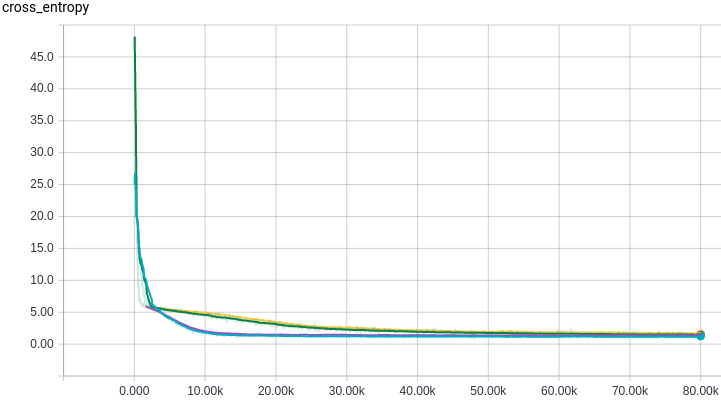
\includegraphics[width=\linewidth]{plots/model1/wteam_onehot/streak-/crossentropy.png}
  \caption{Cross Entropy using no streaks.}\label{fig:wteam-onehot--crossentropy}
\endminipage\hfill
\minipage{0.5\textwidth}
  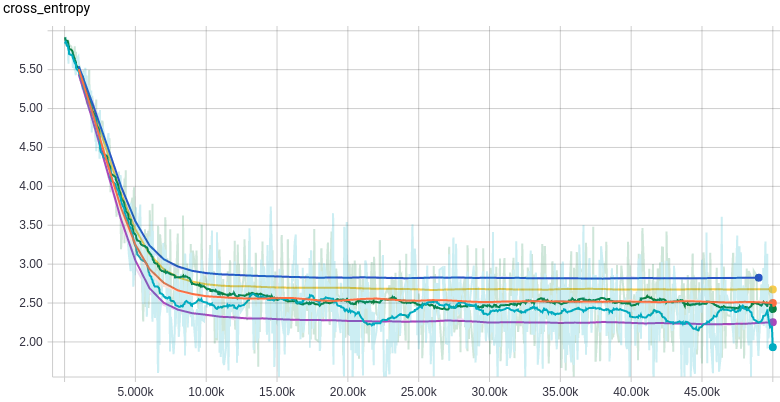
\includegraphics[width=\linewidth]{plots/model1/wteam_onehot/streak-h/crossentropy.png}
  \caption{Cross Entropy using only hot streak.}\label{fig:wteam-onehot-h-crossentropy}
\endminipage\hfill
\minipage{0.5\textwidth}%
  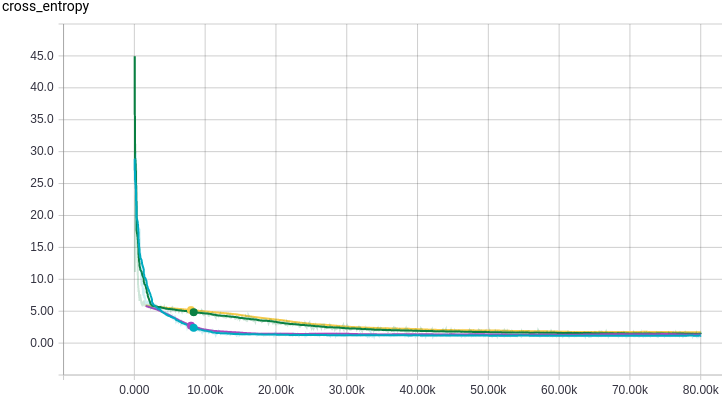
\includegraphics[width=\linewidth]{plots/model1/wteam_onehot/streak-r/crossentropy.png}
  \caption{Cross Entropy using only rival streak.}\label{fig:wteam-onehot-r-crossentropy}
\endminipage
\minipage{0.5\textwidth}%
  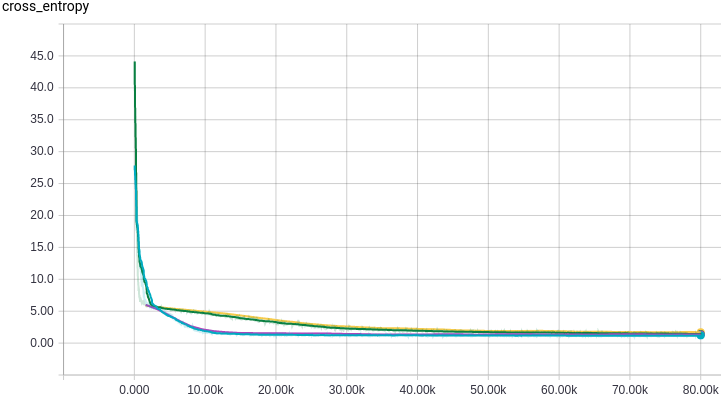
\includegraphics[width=\linewidth]{plots/model1/wteam_onehot/streak-hr/crossentropy.png}
  \caption{Cross Entropy using both hot and rival streaks.}\label{fig:wteam-onehot-hr-crossentropy}
\endminipage
\end{figure}
For both datasets, the cross entropy loss follows an analogous curve to the accuracy where each curve exhibits the same shape and the training loss drops suddenly right at the end (when the accuracy has a sharp improvement).  There does not seem to be any surprises between the accuracy and cross entropy--that is when the cross entropy drops/rises the accuracy increases/decsreases.


Since the accuracy plateaus and the training data doesn't seem to be overfitting, this is evidence that the model is not complex enough and could better generalize using either additional hidden layers and/or more hidden nodes.



\subsection{Predicting Win/Loss Vector}
\label{sec:results-winloss-vector}

\section{Conclusion}
\label{sec:conclusion}


\small{
\nocite{*}
\bibliographystyle{plainnat}
\bibliography{research}
}
\end{document}
